\subsection{Hadamard}%
\label{appendix-hadamard}

Below are several equivalent definitions of the Hadamard generator. Note that the two rightmost definitions do not require any scalar correction.

\begin{figure}[H]
\centering
    \centering
    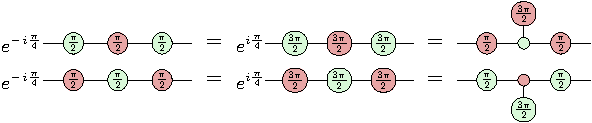
\includegraphics[width=1\textwidth]{chapter-2/hadamard_decomp}
    \caption{Equivalent definitions of the Hadamard generator.}
\end{figure}

%%%

\subsection{Phase Gadgets}%
\label{appendix-phase-gadget-fusion}

We can show how two adjacent phase gadgets fuse using the spider fusion (\ref{spider-fusion}) and bialgebra (\ref{bialgebra}) rules as follows.

\includezxdiagram{chapter-3/phase_gadget_fusion_steps}{0.8}%

%%%

\subsection{Single-Legged Phase Gadgets}%
\label{appendix-phase-gadget-single-leg}

We can show that single-legged phase gadgets are equivalent to $Z$ rotations using the bialgebra (\ref{bialgebra}), spider fusion (\ref{spider-fusion}), state copy (\ref{state-copy}) and identity (\ref{identity}) rules as follows.

\includezxdiagram{chapter-3/phase_gadget_single_leg_steps}{0.8}

%%%

\subsection{Clifford Conjugation Stuff}%
\label{conjugation}

\begin{align*}
    Ce^PC^\dagger &= C \sum_{n=0}^\infty \brac{P^n}{n!} C^\dagger \\
    CP^nC^\dagger &= \sum_{n=0}^\infty \frac{C P^n C^\dagger}{n!} \\
    CP^nC^\dagger &= \sum_{n=0}^\infty \frac{(C P C^\dagger)^n}{n!} \\
    CP^nC^\dagger &= (CPC^\dagger)^n
\end{align*}
